
\subsection*{1.}

\begin{center}
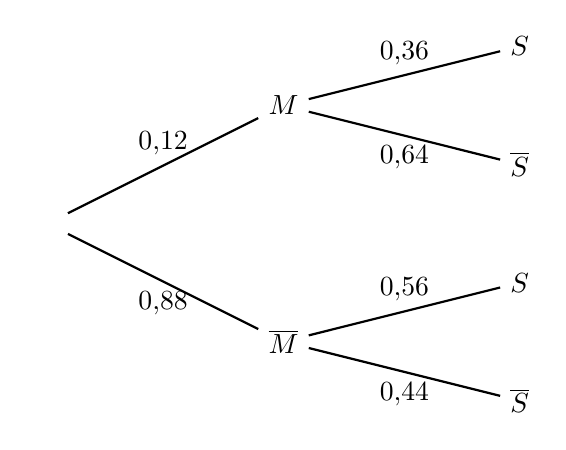
\begin{tikzpicture}[thick, scale=1.5]
\node (P_-1_0) at (-2,-1.5) {$\phantom{A}$};
\node (P_0_0) at (0,-0.5) {$M$};
\draw (P_-1_0) -- (P_0_0) node[midway, above] {$0{,}12$};
\node (P_1_0) at (2,-0) {$S$};
\draw (P_0_0) -- (P_1_0) node[midway, above] {$0{,}36$};
\node (P_1_1) at (2,-1) {$\overline{S}$};
\draw (P_0_0) -- (P_1_1) node[midway, below] {$0{,}64$};
\node (P_0_2) at (0,-2.5) {$\overline{M}$};
\draw (P_-1_0) -- (P_0_2) node[midway, below] {$0{,}88$};
\node (P_1_2) at (2,-2) {$S$};
\draw (P_0_2) -- (P_1_2) node[midway, above] {$0{,}56$};
\node (P_1_3) at (2,-3) {$\overline{S}$};
\draw (P_0_2) -- (P_1_3) node[midway, below] {$0{,}44$};
\end{tikzpicture}
\end{center}

\subsection*{2.}

\paragraph{a.} On calcule :
\begin{align*}
p(M \cap S) &= p(M) \times p_M(S) \\
&= 0{,}12 \times 0{,}36 \\
&= 0{,}0432.
\end{align*}

\paragraph{b.} On a de même :
\begin{align*}
p(\overline{M} \cap S) &= p(\overline{M}) \times p_{\overline{M}}(S) \\
&= 0{,}88 \times 0{,}56 \\
&= 0{,}4928.
\end{align*}

D'après la loi des probabilités totales :
\begin{align*}
p(S) &= p(M \cap S) + p(\overline{M} \cap S) \\
&= 0{,}0432 + 0{,}4928 \\
&= 0{,}536 \neq 0{,}5184.
\end{align*}

\subsection*{3.} Il faut calculer :
\begin{align*}
p_{\overline{S}}(M) &= \dfrac{p(\overline{S} \cap M)}{p(\overline{S})} \\
&= \dfrac{p(M \cap \overline{S})}{p(\overline{S})} \\
&= \dfrac{0{,}12 \times 0{,}64}{1 - 0{,}536} \\
&= \dfrac{0{,}0768}{0{,}464} \approx 0{,}166.
\end{align*}

\subsection*{4.} D'après la question précédente : la probabilité d'être malade sachant que l'on a une activité sportive est égale à :
\begin{align*}
p_S(M) &= \dfrac{p(S \cap M)}{p(S)} \\
&= \dfrac{p(M \cap S)}{p(S)} \\
&= \dfrac{0{,}0432}{0{,}536} \approx 0{,}081. 
\end{align*}

\[
0{,}081 \approx \dfrac{0{,}166}{2},
\]
cette probabilité est environs la moitié de la précédente : la conclusion du journaliste est pertinente.

